\documentclass{article}
\usepackage{setspace}
\usepackage{amsfonts}
\usepackage{amsmath}
\usepackage{graphicx}


\graphicspath{{figures/}}
 
%----------------------------------------------------------------------------------------
%     AUTHORS and ABSTRACT
%----------------------------------------------------------------------------------------

\title{Notes on KdV Results from after General Exam}
\author{Jacob Price}

\begin{document}
\maketitle

\begin{abstract}
In the month since my general examination, I have worked on a lot of ideas relating to constructing reduced order models for KdV. I am expressing them here in detail so that I can pick things up after my vacation without trouble, and so that I can adapt them for future publications. This will be told with colloquial language and in roughly chronological order.
\end{abstract}

%----------------------------------------------------------------------------------------
\section{Time Dependent Coefficients}
%----------------------------------------------------------------------------------------

At the time of the general examination, we had implemented the complete memory approximation up to the third order. The renormalization procedure was completed in the way described in my general exam (very similar to that used in \cite{stinis2015renormalized}).

The first improvement completed after the general exam was the simplification of the code base. The KdV algorithm was simplified into the \verb!KdV_solve.m! file, which could use any of the methods we had previous used. In the past, each of those algorithms had their own Matlab functions, which complicated the file structure.

Allowing a general evolution function to handle each case necessitated the introduction of structure variables, most importantly \verb!simulation_params!, which contains any variables relevant to specific implementations. Different initialization scripts (such as \verb!full_init.m!) are used to specify these parameters before a simulation.

Applying the renormalization procedure to KdV, we found that the coefficients computed were identical to those found by renormalizing Burgers equation. We concluded that this was because they were computed very early in the simulation, before the dispersive term had any appreciable impact upon the dynamics. As far as the renormalization algorithm could tell, it was Burgers equation! The results were unstable.

This suggested to us the possibility of time-dependent renormalization coefficients. Perhaps there is a ``Burgers phase'' as energy drains from the resolved modes, followed by a ``KdV phase'' where energy rebounds back into the resolved modes. Around this same time, Panos and I were discussing the paper \cite{parish2016dynamic}, in which the $t$-model is replaced with a dynamic-$\tau$ model. In the dynamic-$\tau$ model, a time-dependent memory length $\tau$ replaces the $t$ term in the $t$-model. This amounts to a renormalization procedure in which the renormalization constant is itself time-dependent.

Though it seemed daunting, I decided to begin gathering relevant information in order to begin figuring out what sort of time-dependence might be necessary for the renormalization coefficients. The code related to this can be found in the folder \verb!kdv_memory_experiments_mar07!. In order to do so, I needed a fully resolved simulation to compare against. I found that, for $\epsilon=0.1$, the simulation was fully resolved with $N=256$ positive modes. I judged this by the fact that no energy drained from the first $N=128$ positive modes during this simulation (so technically $N=128$ is fully resolved).

\begin{figure}[h]
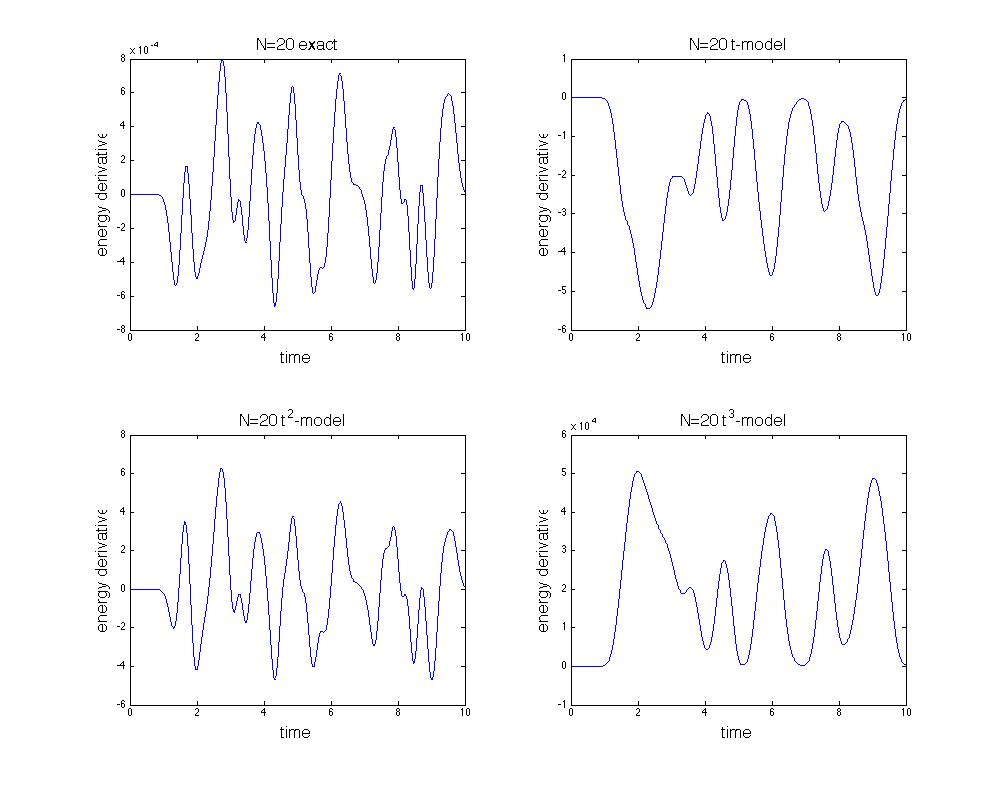
\includegraphics[width=\textwidth]{comparing_energy_derivatives.png}
\caption{The rate of change for the first 20 positive modes of KdV with initial condition $\mathbf{u}(x,0) = \sin(x)$ and $\epsilon=0.1$. The upper left plot is the exact result computed from a fully resolved simulation. The upper right plot depicts the derivative due to the $t$-model term given the exact state vector $\mathbf{u}$. Similarly, the lower left plot depicts the $t^2$-model contribution and the lower right plot depicts the $t^3$-model contribution. Most importantly, note the similarity between the upper left and lower left plots. The results are similar for other resolutions, though the similarity is more dramatic for higher resolutions.}\label{fig:t2_energy_comparison}
\end{figure}

Next, I computed the rate of change of the energy in every individual mode at all times. In the same function, I computed what the contribution to the rate of change of energy in each individual mode due to each term in the complete reduced order model would be given the \emph{exact} state vector, without the $t$-dependence yet included. The descendant of this script is the function \verb!generate_deriv_data_4func!. I found something extremely curious when I plotted the exact energy derivative within a subset of modes alongside the contributions of the complete ROMs to the energy derivative of the same subset. For an example, see Figure \ref{fig:t2_energy_comparison}, though the results are similar for other resolutions.



The result was shocking: it appeared as if the $t^2$-model (without any $t^2$ dependence) very accurately matched the actual rate of energy flow in and out of a set of resolved modes, though with a different scaling on the $y$-axis. This suggested a reduced order model of the form:

\begin{equation}\frac{du_k}{dt} = \sum_{j=0}^M \alpha_j\hat{R}_k^j(\mathbf{u}^0),\label{eq:no_t}
\end{equation}where $R_k^j$ is the contribution of the $j$th term in the complete memory approximation to the $k$th mode. Note that there are renormalization constants $\alpha_j$, but \emph{no} time-dependence, as there typically is. What this means, in reality, is that the ROM is actually of the form:
\[\frac{du_k}{dt} = \sum_{j=0}^M \beta_j(t)t^j\hat{R}_k^j(\mathbf{u}^0)
\]where the time-dependent renormalization constants are $\beta_j = \frac{\alpha_j}{t^j}$.

This on its own has some very interesting implications. What is it about KdV that causes the renormalization constants to have this particular form? Does this say something about the length of the memory kernel in this case? Why did Burgers equation not require any time dependence in its coefficients? As $\epsilon\to0$, KdV converges to Burgers equation. So will these time-dependent coefficients $\beta_j$ converge from $t^{-j}$ dependence to $t^0$ dependence? It seems unlikely that $\epsilon=0.1$ would yield such a special result (in which the time dependence of the renormalization coefficients exactly cancels the time dependence of the rest of the term). This suggests to us that this is due to the singular perturbation nature of the problem. We posit that, for $\epsilon>0$, the time-dependence of the memory terms is $t^{-j}$, while for $\epsilon=0$, the time dependence of the renormalization constants is $t^0$.

In order to confirm how good a fit we could accomplish, I then used a least-squares algorithm to select coefficients for the $t$-model, $t^2$-model and $t^3$-model that minimized the square error between the exact energy flow rate out of the resolved modes and that predicted by a renormalized model of the form (\ref{eq:no_t}). The latest version of code that accomplishes this is \verb!generate_coeffs_4figs!. It was found, as expected, that we can fit the energy derivative into and out of the resolved modes extremely well after rescaling. In addition, we found something else curious: the optimal coefficients seemed to obey a scaling law based upon the resolution of the resolved modes (Figure \ref{fig:loglog_1}).

\begin{figure}[h]
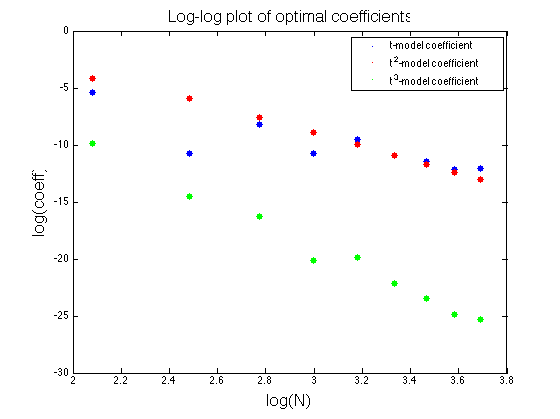
\includegraphics[width=\textwidth]{loglog_1.png}
\caption{A log-log plot of the optimal ROM coefficients found by fitting the derivative of the energy over the range $t\in[0,10]$. Note the general appearance of a scaling law behavior (linear in a log-log plot) in all three terms, but most obviously the $t^2$-model term (red). Note also that the $t$-model and $t^2$-model coefficients are of comparable magnitude, while the $t^3$-model coefficient is several orders of magnitudes smaller. This suggests that a perturbative assumption may be valid.}\label{fig:loglog_1}
\end{figure}

We wondered if we could posit a functional form of $\beta_j(t) = \alpha_j(N) t^{\gamma_j}$ or even $\beta_j(t) = a_j N^{\eta_j}t^{\gamma_j}$. Setting this up as an optimization problem again using the least squares fit, we found that when we used an initial guess \emph{extremely near} the correct choice ($\alpha_j=$ previously found results, $\gamma_j = -j$), it would converge. But otherwise, it diverged. This suggests this is in fact an optimum, but that it is a very deep and narrow minimum. Panos pointed out that this is reminiscent of other critical phenomena. It would be nice to be able to infer the specific form of the scaling laws from the data \emph{a priori}, but this currently seems beyond us.

We then hard-coded in these coefficients to see how well the \emph{actual} energy agrees when we use this ROM for the evolution (Figure \ref{fig:20_3rd_order}). The result was pretty good, and made better when we forced the ROM to begin at a time with low relative error between the exact and predicted energy derivative. Especially as the resolution increased, the energy evolved in a manner very similar to the exact solution. In particular, the phase of oscillation was consistently captured, though often the amplitude was not captured as well as would be desired.

\begin{figure}[h]
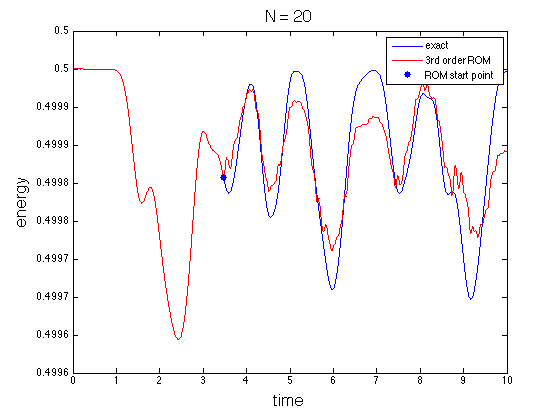
\includegraphics[width=\textwidth]{3rd_order_20.png}
\caption{The energy in the first $N=20$ modes of a KdV simulation with $\mathbf{u}(x,0) = \sin(x)$ and $\epsilon=0.1$. The blue curve is the exact result. The red curve is that predicted by a third-order ROM with optimal coefficients fit to minimize the difference between the exact energy derivative and that predicted by the ROM. The blue dot indicates the location at which the ROM begins acting (chosen as the point at which the ROM energy derivative has the lowest relative error). Note that it gets the phase quite accurately, but misses the amplitude to some degree.}\label{fig:20_3rd_order}
\end{figure}

Lower resolutions did not have as impressive results (Figure \ref{fig:8_3rd_order}), but there certainly seemed to be something important and deep at work.

\begin{figure}[h]
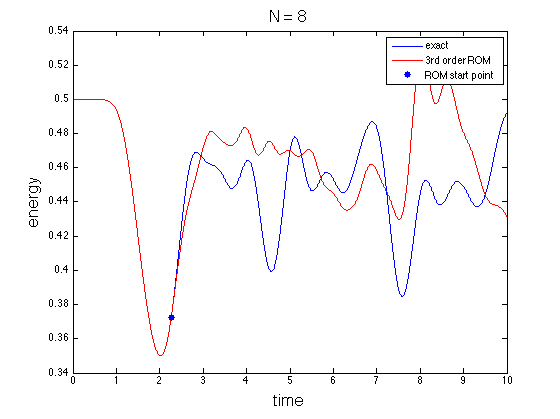
\includegraphics[width=\textwidth]{3rd_order_8.png}
\caption{The energy in the first $N=8$ modes of a KdV simulation with $\mathbf{u}(x,0) = \sin(x)$ and $\epsilon=0.1$. The blue curve is the exact result. The red curve is that predicted by a third-order ROM with optimal coefficients fit to minimize the difference between the exact energy derivative and that predicted by the ROM. The blue dot indicates the location at which the ROM begins acting (chosen as the point at which the ROM energy derivative has the lowest relative error). Note that it appears to capture the phase, but does a very poor job of approximating the amplitude (much worse than the $N=20$ case in Figure \ref{fig:20_3rd_order}).}\label{fig:8_3rd_order}
\end{figure}

\section{Derivation of ROMs}

We hypothesized that the errors would be improved by the addition of the fourth order term. There were a few reasons to suspect this. First, we found empirically, that the contribution of the $t$-model term was always negative (this can be proven) and the $t^3$-model term contribution seemed to be always positive. The $t^2$-term did not have a fixed sign, and seemed to most accurately approximate the energy derivative. We posited that the $t^4$-model term would also have no fixed sign, and that it was important for capturing the details. We hypothesized that the unclear scaling laws for the $t$-model and $t^3$-model terms came from them attempting to account for the behavior of the missing $t^4$-model term.

Rather than computing the $t^4$-model term by hand, which would likely incur errors, we constructed a Mathematica document to do so. The resulting Mathematica document can compute complete memory approximations of any PDE up to any order. One can substitute in the definitions for $\mathcal{L}$ and $P$ associated with our problem to get the specific KdV complete memory terms. This alone is a significant development that will greatly help investigations into reduced order models of other equations. These documents are saved as \verb!General Memory Terms! and \verb!KdV Symbolic Memory Computation!.

The $t^4$-model term was not simple, but the Mathematica notebooks made it much easier to compute its form and organize it. This made the implementation as pain-free as possible, and the resulting functions (\verb!t4model_term_complete!, \verb!renormalized_4th_order_complete! and related) seem to be possibly bug-free.

\section{Fitting through the 4th order}

As predicted, the $t^4$ model did not have a fixed sign (Figure \ref{fig:energy_deriv_4}). In fact, it seemed to, like the $t^2$-model contribution, roughly echo the exact result. We were hopeful that, with this term included, we could better approximate the energy derivative with a least squares fit.

\begin{figure}[h]
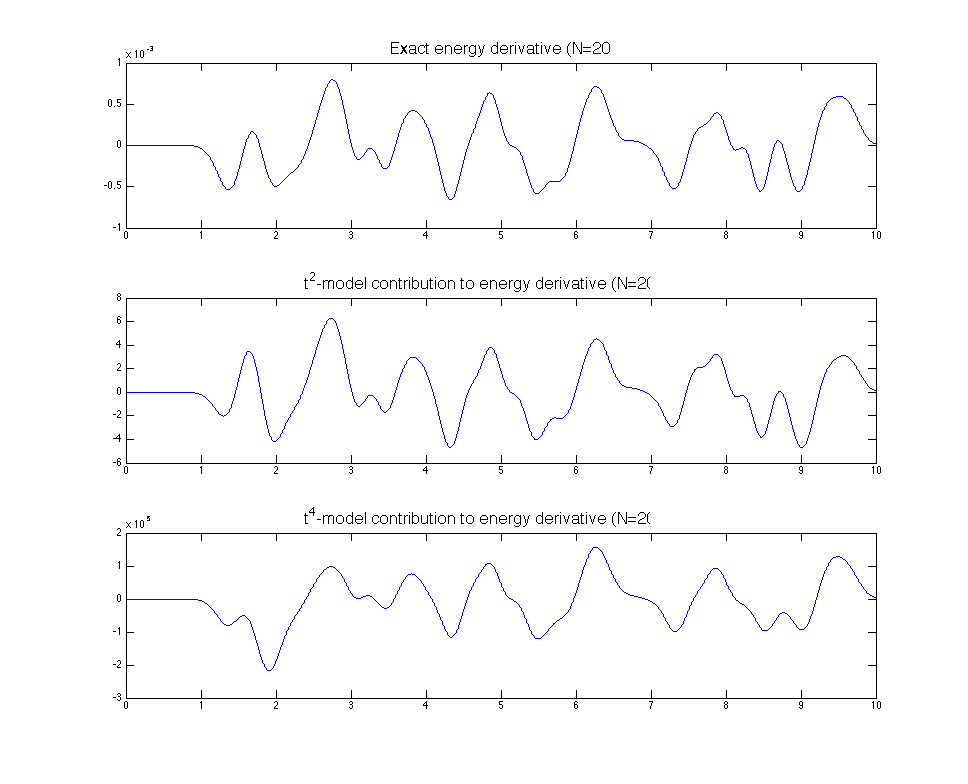
\includegraphics[width=\textwidth]{comparing_derivatives_2.png}
\caption{The rate of change for the first 20 positive modes of KdV with initial condition $\mathbf{u}(x,0) = \sin(x)$ and $\epsilon=0.1$. The upper plot is the exact result computed from a fully resolved simulation. The middle plot depicts the $t^2$-model contribution and the lower plot depicts the $t^4$-model contribution. Note that the $t^4$-model contribution is also not of fixed sign, and seems to be in phase with the exact result.}\label{fig:energy_deriv_4}
\end{figure}

The new fit is noticeably better, but not dramatically so, especially for lower resolutions (Figures \ref{fig:least_squares_3_vs_4} and \ref{fig:least_squares_3_vs_4_8}). This suggests that it was not the missing 4th order term that was interfering with the reduced order models of low-resolutions.



\begin{figure}[h]
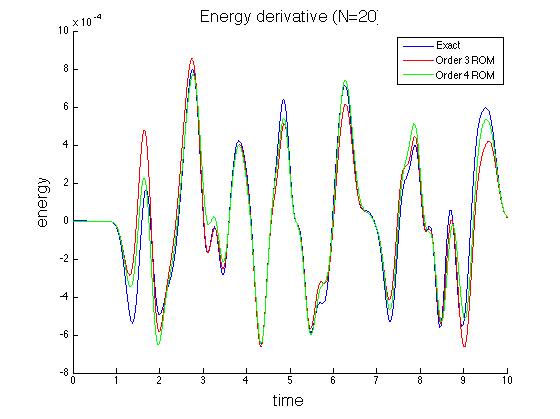
\includegraphics[width=\textwidth]{4th_order_fit.png}
\caption{The least-squares fits of the order 3 ROM and the order 4 ROM for the derivative of the energy in the first 20 modes. Note that the 4th order ROM approximates the exact solution better than the 3rd order ROM, but not dramatically so.}\label{fig:least_squares_3_vs_4}
\end{figure}

\begin{figure}[h]
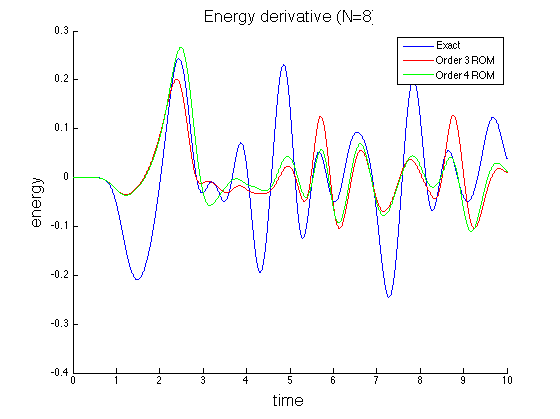
\includegraphics[width=\textwidth]{4th_order_fit_8.png}
\caption{The least-squares fits of the order 3 ROM and the order 4 ROM for the derivative of the energy in the first 8 modes. Note that neither ROM approximates the derivative well, suggesting that the missing 4th order term was not responsible for the errors.}\label{fig:least_squares_3_vs_4_8}
\end{figure}

An additional exciting result, however, was the vast improvement of the scaling law behavior. Low-resolution modes ($N=8$ and $N=12$) did not seem to fit the pattern, but once they were removed, the results were impressive (Figure \ref{fig:scaling_laws}). It appears we were correct that the $t$-model and $t^3$-model were inefficiently being used to account for both their role and that of the $t^4$-model term. We also notice that the perturbative expansion assumptions seem to hold: higher order terms in the memory expansion receive smaller coefficients. This suggests that the addition of more terms will likely lead to diminishing returns, suggesting that additional terms will not alleviate the problems with the low-resolution models. We see also that the optimal $t$-model and $t^2$-model terms are of similar magnitude, and the $t^3$-model and $t^4$-model terms of of comparable magnitude. Perhaps these terms must be added in pairs, which was a result Panos encountered in his Burgers equation studies.



\begin{figure}[h]
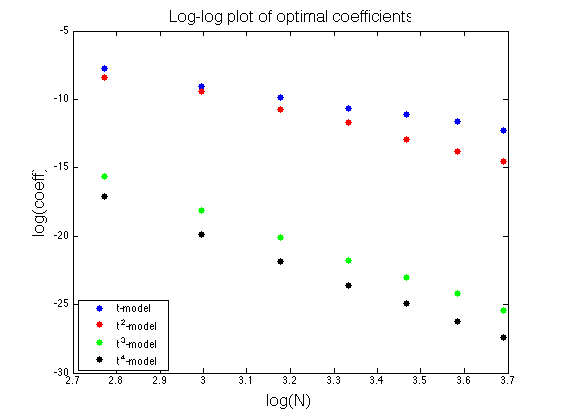
\includegraphics[width=\textwidth]{loglog_2.png}
\caption{Log-log plot of the optimal coefficients for each of the first four terms in a complete memory approximation of Kdv. There is clear evidence of a scaling law behavior for each coefficient.}\label{fig:scaling_laws}
\end{figure}

Using the same hard-coding algorithm, we found that the results improved, but not dramatically, especially for low resolutions (Figures \ref{fig:20_4th_order} and \ref{fig:8_4th_order}). In addition, we began thinking about how these results could be generalized. In a realistic simulation, we would not have access to the exact solution up to time $t=10$, as was used to compute these coefficients. It would be better if the amount of time the exact solution is needed were shorter. Perhaps up to a time that a full model of only double the reduced model were still fully resolved. One hopes that the optimal coefficients might be accessible after a shorter time period.

\begin{figure}[h]
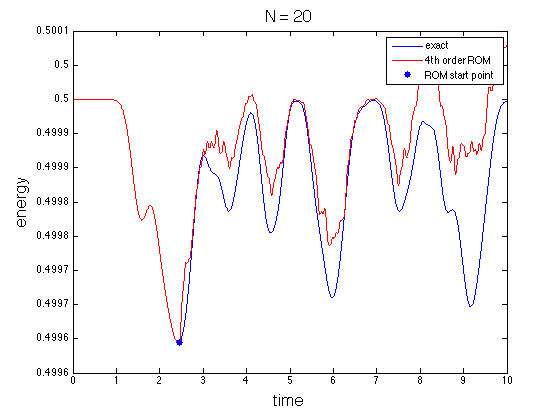
\includegraphics[width=\textwidth]{4th_order_20.png}
\caption{The energy in the first $N=20$ modes of a KdV simulation with $\mathbf{u}(x,0) = \sin(x)$ and $\epsilon=0.1$. The blue curve is the exact result. The red curve is that predicted by a fourth-order ROM with optimal coefficients fit to minimize the difference between the exact energy derivative and that predicted by the ROM. The blue dot indicates the location at which the ROM begins acting (chosen as the point at which the ROM energy derivative has the lowest relative error). Note that it appears to capture the phase, and does a decent job of approximating the amplitude.}\label{fig:20_4th_order}
\end{figure}

\begin{figure}[h]
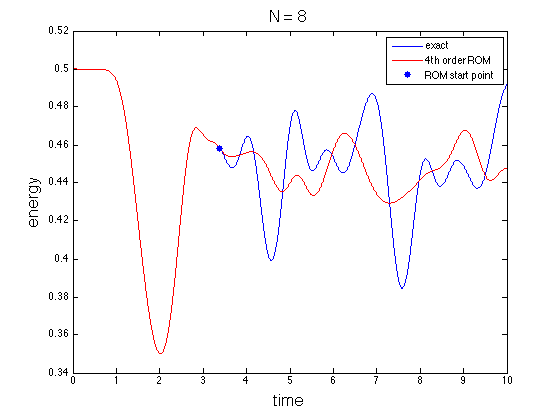
\includegraphics[width=\textwidth]{4th_order_8.png}
\caption{The energy in the first $N=8$ modes of a KdV simulation with $\mathbf{u}(x,0) = \sin(x)$ and $\epsilon=0.1$. The blue curve is the exact result. The red curve is that predicted by a fourth-order ROM with optimal coefficients fit to minimize the difference between the exact energy derivative and that predicted by the ROM. The blue dot indicates the location at which the ROM begins acting (chosen as the point at which the ROM energy derivative has the lowest relative error). Note that it appears to capture the phase, but still does a very poor job of approximating the amplitude.}\label{fig:8_4th_order}
\end{figure}

We thus plotted these coefficients computed from a least squares fit over $t\in[0,x]$ where $x\in[2,10]$. We were hopeful that the coefficients would be stable over time, and that they would ``lock in'' early. Indeed, we found this to be the case (Figure \ref{fig:20_coeffs}), even for the problematic low-resolution cases. In addition, it appeared that the coefficients for $t$ and $t^3$ were closely related, as were the coefficients for $t^2$ and $t^4$.


\begin{figure}[h]
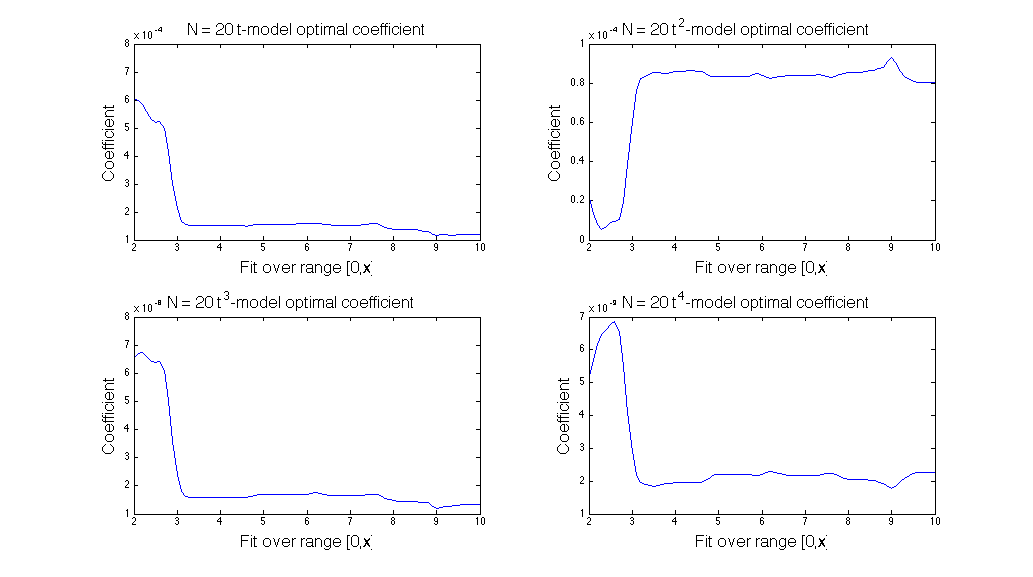
\includegraphics[width=\textwidth]{coeffs_20.png}
\caption{The optimal coefficients for the $N=20$ ROM. The fits were computed in a least-squares sense to match the energy derivative over a range of $t\in[0,x]$ where $x$ varied from 2 to 10. We see that the coefficients seem to ``lock in'' after about $t=3$. This coincides with the point after the first energy drain and rebound have been completed. The results are similar for other resolutions. Notice also that the plots for the $t$ and $t^3$ coefficients appear extremely similar, as do the plots for the $t^2$ and $t^4$ coefficients (if you multiply the $t^4$ curve by -1).}\label{fig:20_coeffs}
\end{figure}

We hypothesized also that the coefficients themselves might need to be time dependent. For this reason, we computed the optimal coefficients using a sliding window of $[x-a,x]$ where $a$ is some constant. If the optimal coefficients stabilize upon the same values seen above, it would suggest that perhaps there are two phases. Unfortunately, the results were inconclusive, though the similarity between the $t$ and $t^3$ terms and the $t^2$ and $t^4$ terms persisted (Figure \ref{fig:20_coeffs_2}).

Another way in which the cost of computing these terms could be considered worthwhile is if the accuracy of simulation persists long after $t=10$. I do not have these plots on hand, and they take too long to produce for me to have them ready today. However, we found that the accuracy does indeed persist after $t=10$, though not indefinitely.

\begin{figure}[h]
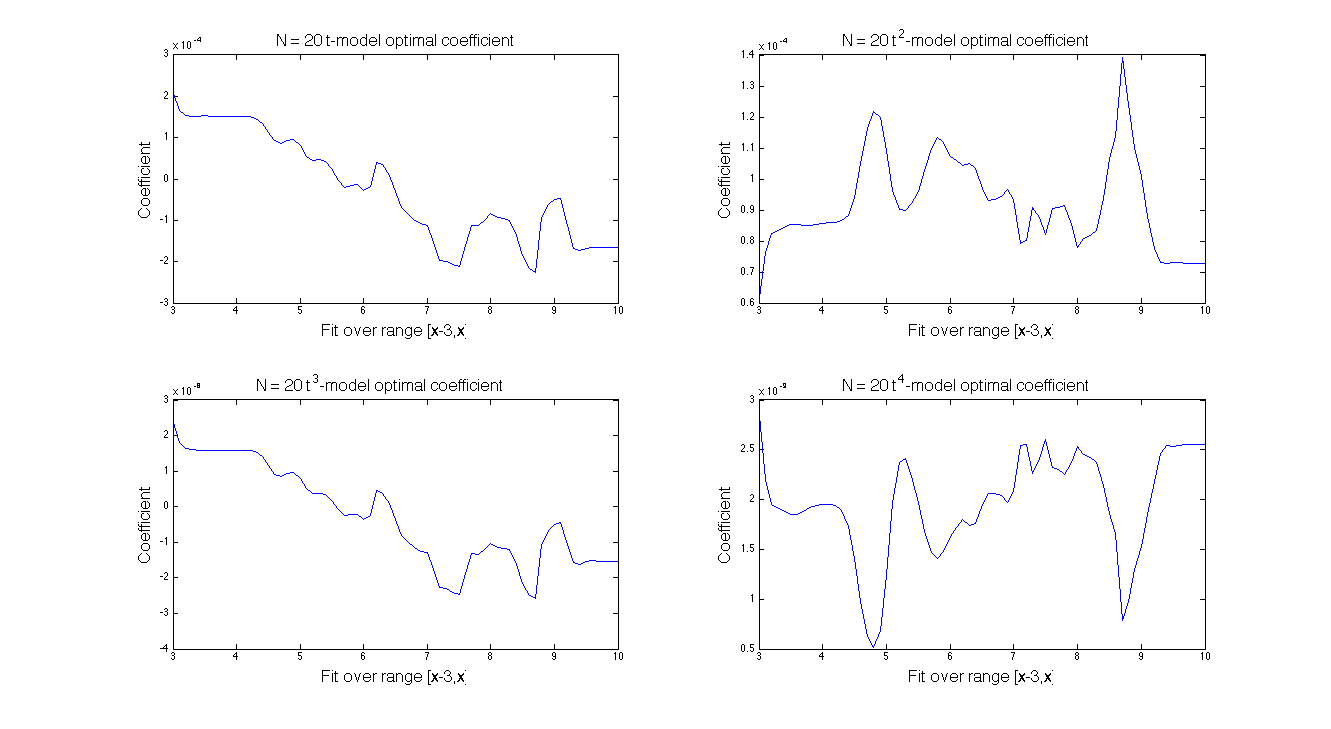
\includegraphics[width=\textwidth]{coeffs_20_2.png}
\caption{The optimal coefficients for the $N=20$ ROM. The fits were computed in a least-squares sense to match the energy derivative over a range of $t\in[x-3,x]$ where $x$ varied from 3 to 10. We no longer see any clear ``locking in,'' casting doubt upon the previous results. It seems a good deal of of data is needed to find the aforementioned stable results. What we do notice, however, is that the $t$ and $t^3$ model fits seem to be highly related to each other, as do the $t^2$ adn $t^4$ coefficients (consider flipping the $t^4$ plot over).}\label{fig:20_coeffs_2}
\end{figure}

\section{$k$-dependent Coefficients}

I was next curious about why, even when the derivative of the energy was almost exactly matched by the ROM, the energy during the evolution would deviate from the exact result almost immediately. If there is very little visible difference between the two, I would not expect the errors to be incurred so quickly, but rather to develop over time. Indeed, the fact that the error fit sometimes underestimated and sometimes overestimated the derivative suggested that in general the agreement should be rather good in the actual evolution.

As a working theory, I wondered whether the net flow in and out of the resolved modes was being well matched, but that the energy flow into and out of individual resolved modes was being poorly represented. In this case, after a few steps in the simulation, the underlying state vector $\mathbf{u}$ would have deviated from the correct state. Our fits are based on the ROM being fed the correct state vector, so we would enter uncharted territory when this error occurred, and have no guarantee of producing reasonable results.

I plotted the energy derivative in individual modes (Figure \ref{fig:individual_modes}), and found that they were indeed being poorly represented, even in the case where the net energy was well approximated. With my suspicions confirmed, I wondered if constructing a reduced order model that respected the dynamics of the individual modes would yield an ROM that tracked the net energy better, while also capturing the real-space dynamics accurately.

\begin{figure}[h]
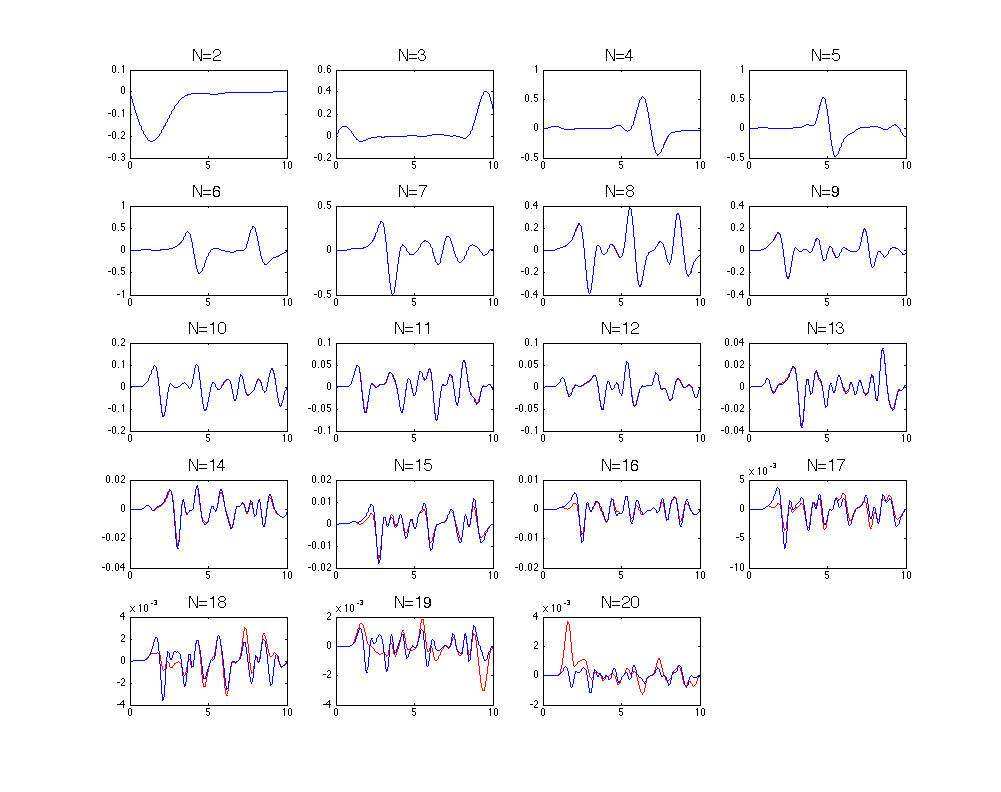
\includegraphics[width=\textwidth]{individual_modes.png}
\caption{The energy derivative of individual modes exactly (blue) and for the $N=20$ ROM with optimal coefficients for the net energy derivative (red). For low resolution modes, the ROM results are almost indistinguishable from the exact results. This is because the memory terms are quite small for low resolution modes, and the dynamics of the low wavenumber modes are dominated by the Markov term. For modes near the end of the resolved range, which are the ones that have significant memory effects, the dynamics of the individual modes are not well captured, though the net flow in and out of the resolved modes is good (Figure \ref{fig:least_squares_3_vs_4}).}\label{fig:individual_modes}
\end{figure}

It seemed unrealistic to expect a good fit for individual modes when we only had four coefficients to fit. Instead, I elected to allow the renormalization coefficients to depend upon the wavenumber $k$ as well. Thus, the reduced order model would now have the form:
\begin{equation}\frac{du_k}{dt} = \sum_{j=0}^M \alpha_j(k)\hat{R}_k^j(\mathbf{u}^0).\label{eq:k}
\end{equation}

I selected these coefficients $\alpha_j(k)$ using a least-squares fit that took into account the square error within each individual mode over the full $t\in[0,10]$ time range. The results captured the individual modes extremely accurately (Figure \ref{fig:individual_modes_k}), but does not do as well on the net energy flow into and out of the resolved modes (Figure \ref{fig:k_dependent_net}).

\begin{figure}[h]
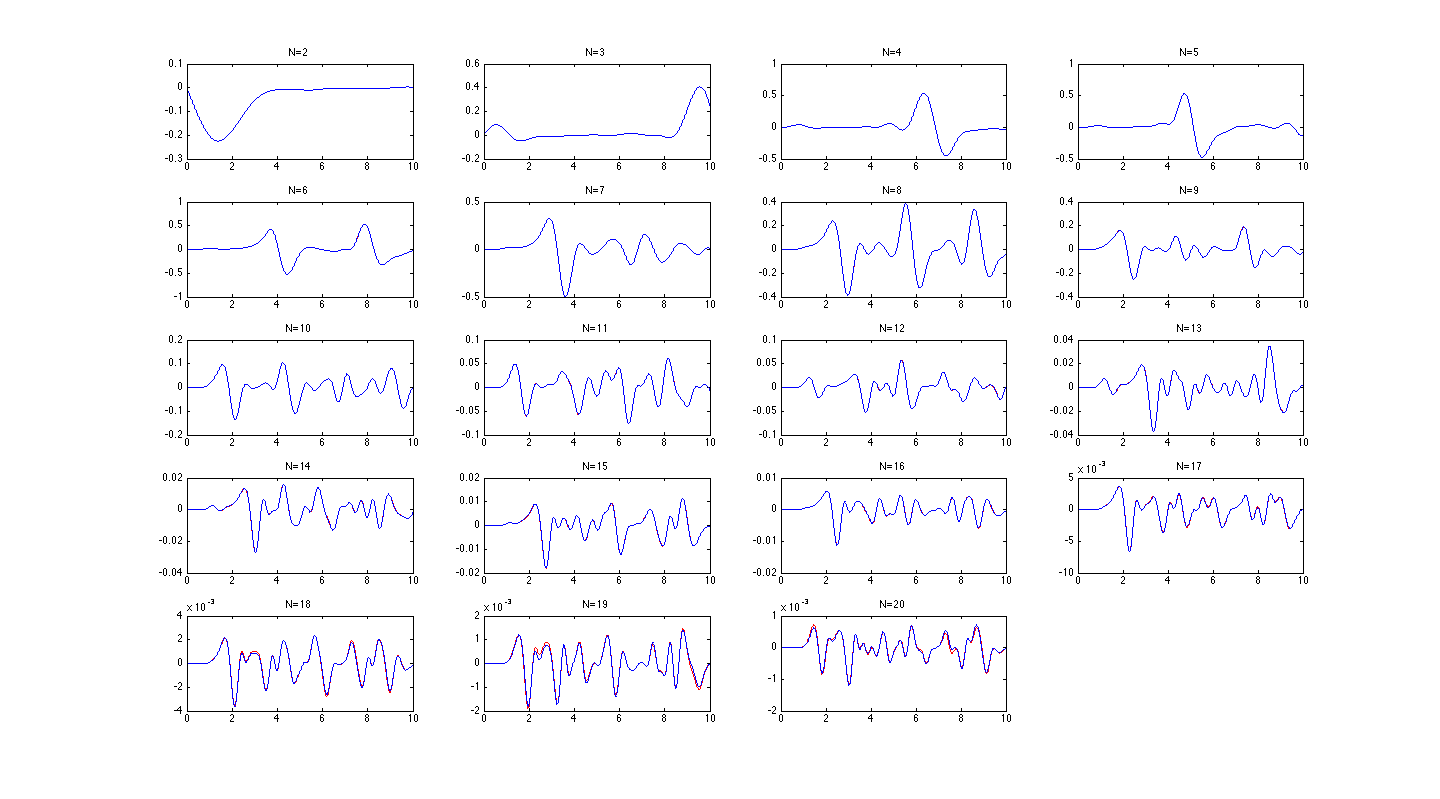
\includegraphics[width=\textwidth]{individual_modes_k.png}
\caption{The energy derivative of individual modes exactly (blue) and for the $N=20$ ROM with optimal coefficients for the energy derivative of each mode (red). The fit is so good that it is almost impossible to see a difference in any of the modes.}\label{fig:individual_modes_k}
\end{figure}

\begin{figure}[h]
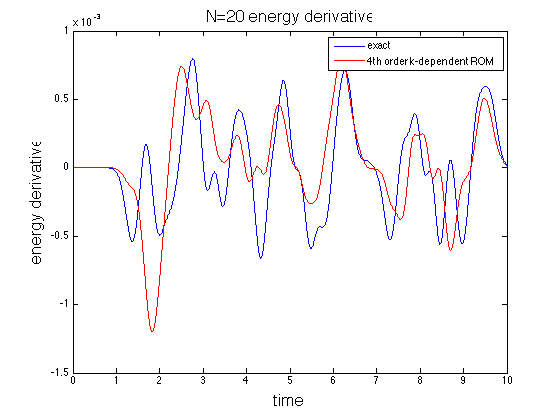
\includegraphics[width=\textwidth]{k_dependent_20.png}
\caption{The net energy derivative in the first $N=20$ modes exactly (blue) and for the $N=20$ ROM with optimal coefficients for the energy derivative of each mode (red). Though each individual mode is fit exceedingly well, the net result is quite inaccurate.}\label{fig:k_dependent_net}
\end{figure}

Using these coefficients to actually evolve the system led to predictable results. The net energy in the system was not captured well at all (Figure \ref{fig:k_dependent_evolution}). However, the real space solution remained \emph{extremely} accurate over the full simulation (Figure \ref{fig:real_space_k}).

\begin{figure}[h]
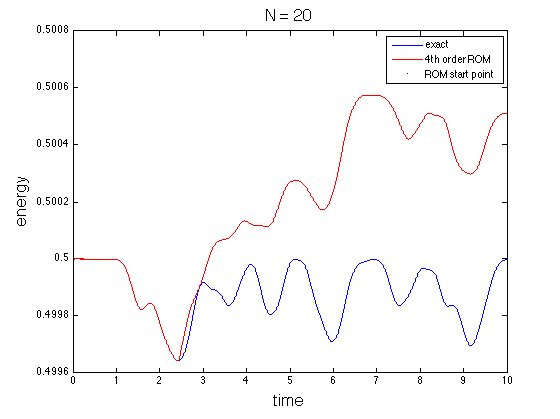
\includegraphics[width=\textwidth]{k_dependent_20_energy.png}
\caption{The energy in the first $N=20$ modes in an exact simulation (blue) and in a simulation that optimizes the energy derivative of each individual mode using $k$-dependent renormalization coefficients. Note that the phase and general shape is quite good, but otherwise the agreement leaves much to be desired.}\label{fig:k_dependent_evolution}
\end{figure}

\begin{figure}[h]
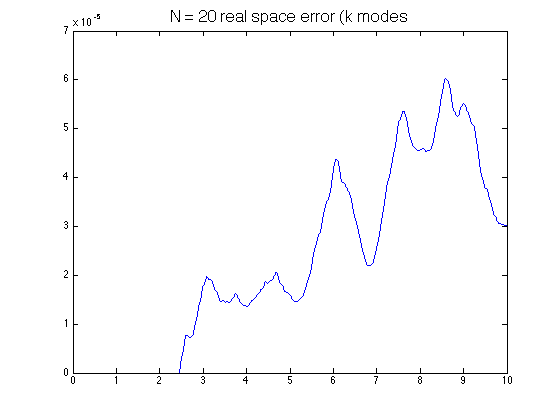
\includegraphics[width=\textwidth]{real_space_20.png}
\caption{The relative error of the real space solution computed with the $N=20$ ROM with $k$-dependent coefficients fit to match the energy derivative of individual modes. Computed as the two-norm of the difference between the ROM real space solution and the exact real space solution (confined to only the first $N=20$ modes) divided by the two-norm of the exact solution. Note that the global error never exceeds 1e-4, which is tremendously impressive.}\label{fig:real_space_k}
\end{figure}

The results are similar for other discretizations. In general, $N=8$ and $N=12$ have poor results, but for $N=16$ and larger, the real space solution is excellent and the total energy is less impressive. The results improve in both metrics as $N$ increases.

In order to improve the net energy evolution, we sought a compromise. We allowed the coefficients to be fit both to the individual modes and the net energy flow in a least squares sense (Figures \ref{fig:individual_modes_both_k} and \ref{fig:k_dependent_both_net}). The result is a compromise: less accuracy in real space, but improved results in the net energy evolution (Figures \ref{fig:both_evolution} and \ref{fig:both_real_space}). At present, these are the best results we have found.

\begin{figure}[h]
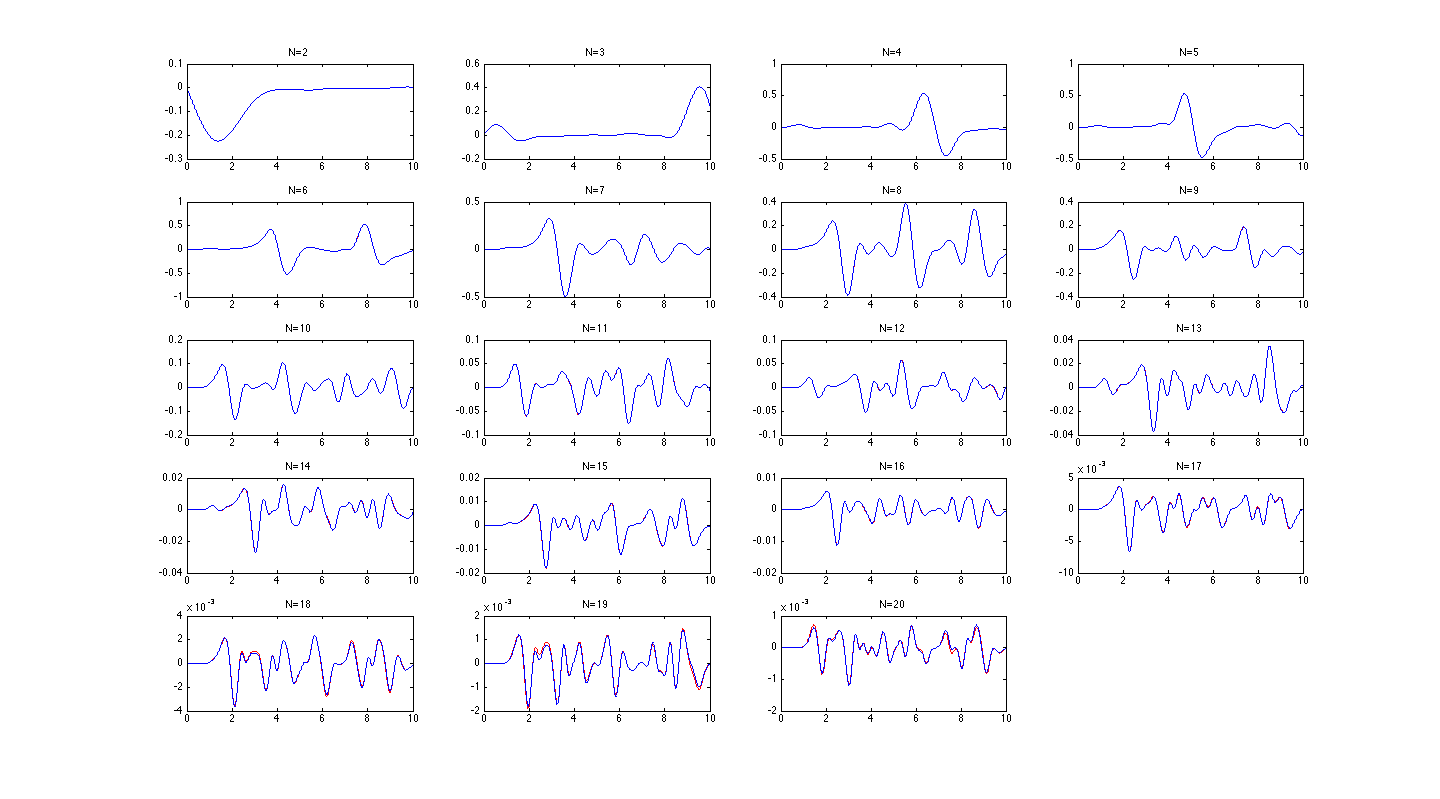
\includegraphics[width=\textwidth]{individual_modes_k.png}
\caption{The energy derivative of individual modes exactly (blue) and for the $N=20$ ROM with optimal coefficients fit to both the energy derivative of each mode and the net energy derivative in and out of the resolved modes (red). The fit is still tremendously good, almost indistinguishable from the previous result.}\label{fig:individual_modes_both_k}
\end{figure}

\begin{figure}[h]
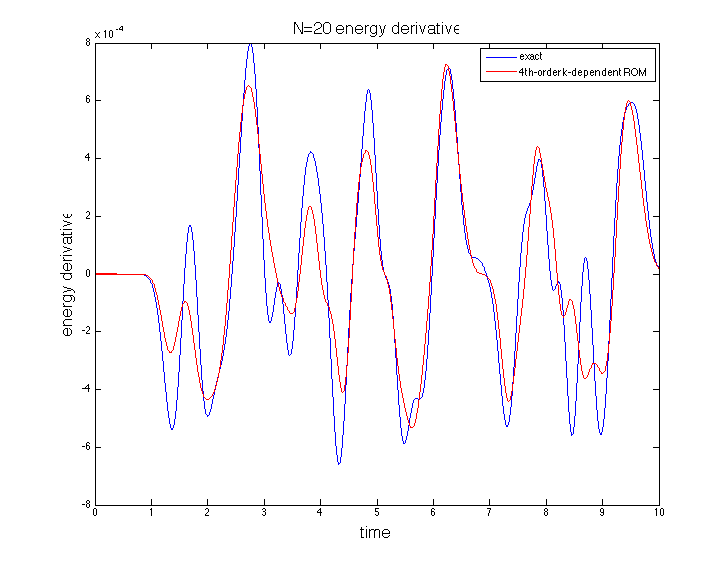
\includegraphics[width=\textwidth]{energy_both.png}
\caption{The net energy derivative in the first $N=20$ modes exactly (blue) and for the $N=20$ ROM with optimal coefficients fit to both the energy derivative of each mode and the net energy derivative in and out of the resolved modes (red). The net energy flow is far more accurate.}\label{fig:k_dependent_both_net}
\end{figure}

\begin{figure}[h]
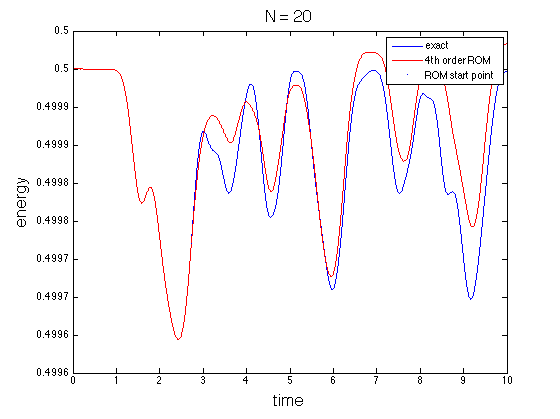
\includegraphics[width=\textwidth]{both_energy_evolution.png}
\caption{The energy in the first $N=20$ modes in an exact simulation (blue) and in a simulation that optimizes the energy derivative of each individual mode and in aggregate using $k$-dependent renormalizaiton coefficients. This agreement is far improved over Figure \ref{fig:k_dependent_evolution}.}\label{fig:both_evolution}
\end{figure}

\begin{figure}[h]
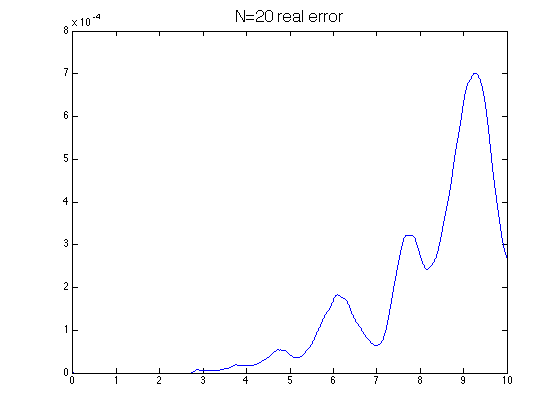
\includegraphics[width=\textwidth]{both_real_space.png}
\caption{The relative error of the real space solution computed with the $N=20$ ROM with $k$-dependent coefficients fit to match the energy derivative of individual modes and the net energy change. Computed as the two-norm of the difference between the ROM real space solution and the exact real space solution (confined to only the first $N=20$ modes) divided by the two-norm of the exact solution. Note that the global error never exceeds 1e-3. Thus, the error is not significantly higher than the model fit only to the individual modes.}\label{fig:both_real_space}
\end{figure}

\section{Analysis of the $k$-dependent coefficients}

Now that we have reached a reduced order model that performs well under both metrics (for $N=16$ or larger), we return to the problem of how to compute these coefficients from less data. From here on, we will only consider the results for $N=16$ and larger.

First, we wonder if there is any sort of common pattern or predictability amongst the optimal coefficients. Indeed, there is some. First, the $t^2$-model coefficients associated with every wavenumber are negative. Similarly, the $t^4$-model coefficients associated with every wavenumber are positive. The $t$-model and $t^3$-model coefficients do not have a fixed sign, nor a visible pattern in the signs.

All four coefficients, however, appear to obey a scaling law for each individual mode. The $t^2$ and $t^4$ coefficients demonstrate this more clearly, while the $t$ and $t^3$ coefficients follow a more general trend (Figure \ref{fig:k_scaling}). The more dramatic scaling laws for the $t^2$ and $t^4$ terms, along with their fixed sign suggest to me that they may be more important. One future thing I would like to try is conducting a fit that involves only the $t^2$ and $t^4$ terms.

\begin{figure}[h]
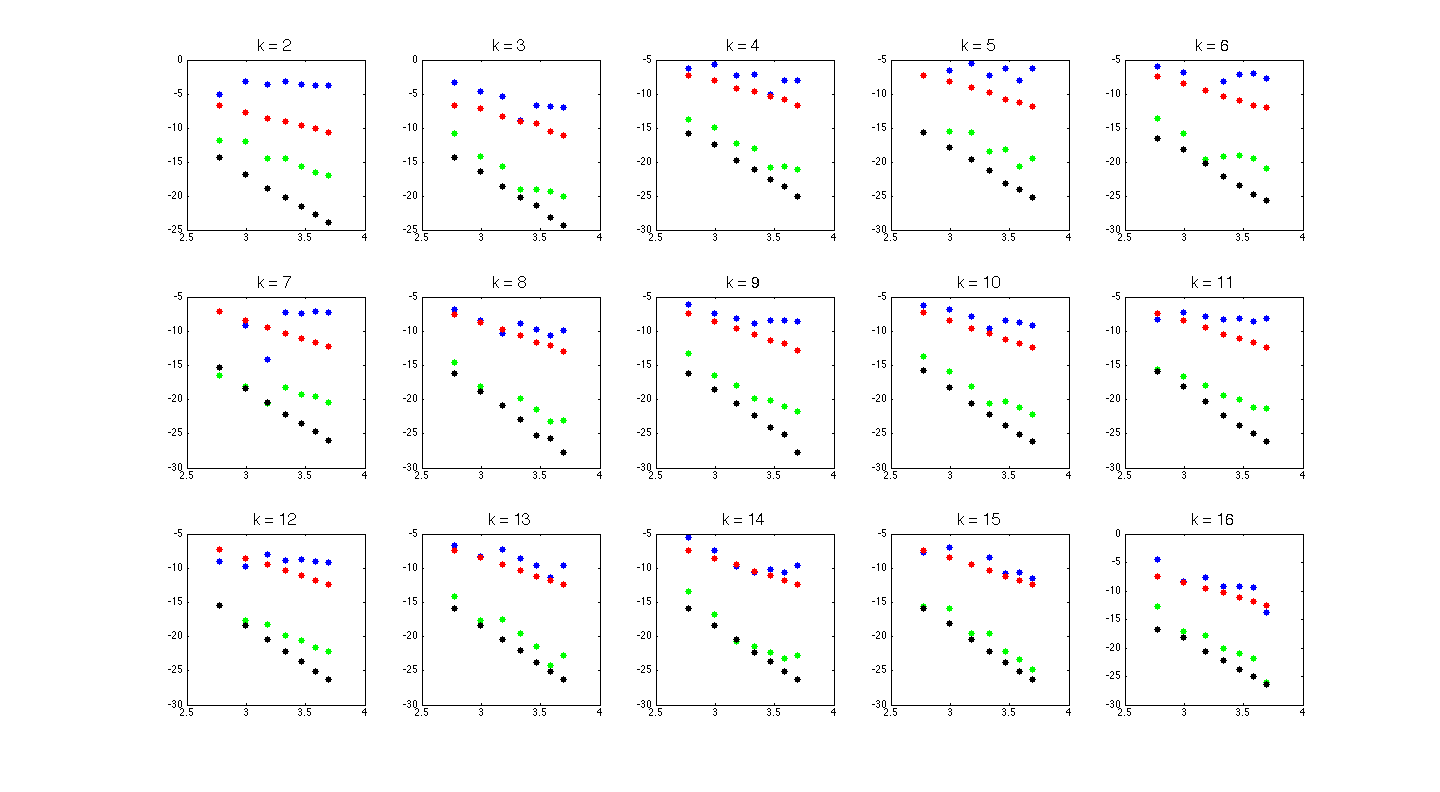
\includegraphics[width=\textwidth]{k_scaling_laws.png}
\caption{Log-log plots of the absolute values of the optimal coefficients for individual modes fit to both the energy derivative of the individual modes and the net energy derivative. The $x$-axis of each plot is $\log(N)$ while the $y$-axis is $\log(\text{coeff})$. The $t$-model coefficients (blue) and $t^3$-model coefficients (green) show a general downward trend. The $t^2$-model coefficients (red) and the $t^4$-model coefficients (black) show a much more obvious scaling law.}\label{fig:k_scaling}
\end{figure}

It is also prudent to study how the coefficients vary across the wavenumbers. If we hope to construct these coefficients without the full solution, any patterns we can uncover would be helpful. Indeed, we find the coefficients dependence on $k$ is quite predictable. Figure \ref{fig:wavenumber_dependence} depicts the results for $N=20$, but other resolutions have a similar structure. This suggests that the $k$-dependent coefficients are not so $k$-dependent after all. In fact, for wavenumbers larger than about $k=5$, the $t^2$ and $t^4$ have approximately fixed values, while the $t$ and $t^3$ terms are essentially zero. It is only in the very small wavenumbers that meaningful differences appear. We once again the curiously strong relationship between the coefficients of the $t$ and $t^3$ terms and the $t^2$ and $t^4$ terms.

The existence of patterns, both in the specific wavenumber dependence and in the scaling between resolutions, suggest a rich structure in the renormalization coefficients. If this structure can be characterized, it is possible we will be able to infer these coefficients, or write formulae for them, that would extend to other systems for which we do not have the exact solution. In particular, if we can find some sort of scaling law in $\epsilon$, it is possible we could extend these results into domains for which the exact solution is not accessible. This is a short-term goal to work on.

The less predictable behavior of the $t$ and $t^3$ coefficients, in comparison to the $t^2$ and $t^4$ coefficients (which have a fixed sign and a strict scaling law), is notable. I suspect there is more to be learned about the odd-power expansions.

\begin{figure}[h]
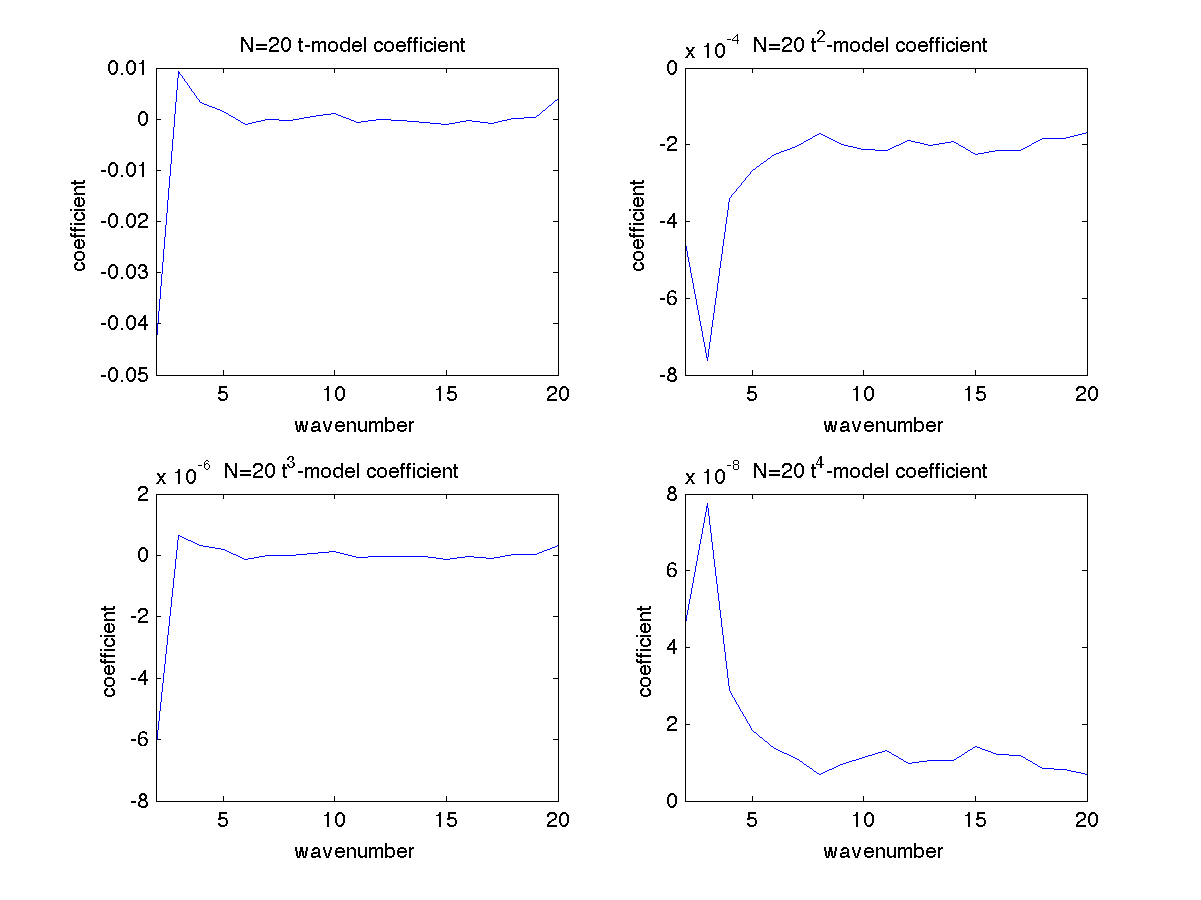
\includegraphics[width=\textwidth]{N20_k_coeffs.png}
\caption{Dependence of optimal coefficients on the wavenumber. Note that the optimal coefficient for all four models is largely independent on the wavenumber, except for the very small wavenumbers. Observe also that the optimal $t^2$ coefficient for large wavenumbers is a fixed negative number, and the optimal $t^4$ coefficient for large wavenumbers is a fixed positive number. The $t$ and $t^3$ optimal coefficients seem to be zero for large wavenumbers. This suggests that the $t$ and $t^3$ models may only be needed for the first few wavenumbers. We also, once again, see the similarity between the $t$ and $t^3$ coefficients and between the $t^2$ and $t^4$ coefficients.}\label{fig:wavenumber_dependence}
\end{figure}

\section{Burgers equation}

I attempted to apply the methods described in the above document to Burgers equation as well. I will describe the results in words here, as I am not certain there was much worthwhile gained (besides insight).

For an ``exact solution,'' I used the upstream method on a very fine grid. I plotted (exactly) the net energy flowing out of resolved modes, and the contributions to the same of the different terms in the ROM (without $t$-dependence). The contributions of the ROM terms all looked roughly similar to the exact net energy flow, though with different scalings (and sometimes different signs). Including the $t$-dependence, the agreement between the $t$-model and the exact derivative, in particular, was quite clear. However, to begin I focused on fitting the data without $t$-dependence.

Fitting these data to single coefficients for each ROM, I found the coefficients for the $t$, $t^2$, $t^3$, and $t^4$ models (again considering $N=16$ or larger) were of fixed sign and obeyed very strict scaling laws (Figure \ref{fig:burgers_loglog}). When using these coefficients to actually evolve the system, the energy agreement was quite good, even when the ROM was turned on at the same time as would have triggered the old renormalization method (Figure \ref{fig:burgers_20}). There was some instability and oscillations, especially for higher resolutions, but the results were quite impressive othrewise. This is particularly curious because the previous renormalization methods included the additional $t$ dependence, yet this method seemed to perform quite well.

\begin{figure}[h]
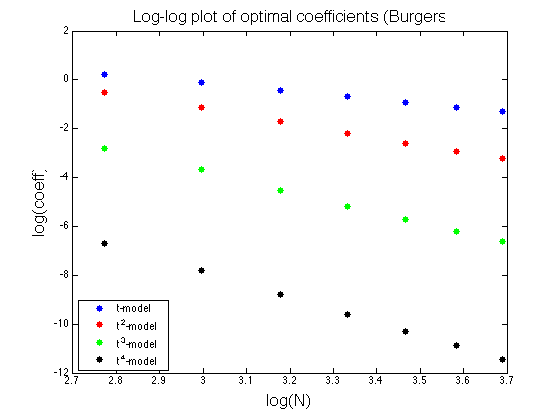
\includegraphics[width=\textwidth]{burgers_loglog.png}
\caption{Scaling law behavior of optimal coefficients fit to Burgers equation over $t\in[0,10]$ with no built in $t$-dependence. Note that all four reduced order models obey a strict scaling law, and that the perturbation assumption is satisfied. In addition, the coefficients are of fixed sign for a given term.}\label{fig:burgers_loglog}
\end{figure}

\begin{figure}[h]
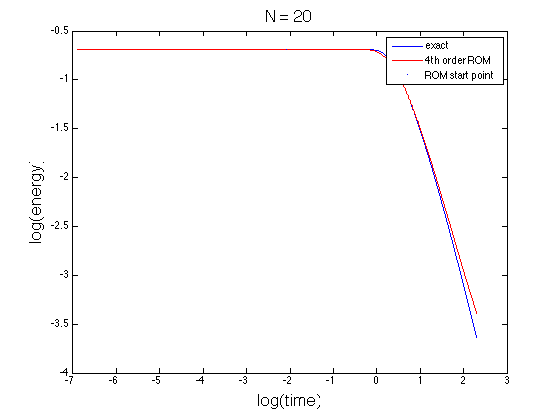
\includegraphics[width=\textwidth]{burgers_20.png}
\caption{Log-log energy evolution of the first $N=20$ modes of Burgers equation computed ``exactly'' (blue) and from a 4th order ROM with no time dependence and coefficients determined by fitting the energy derivative of those 20 modes over $t\in[0,10]$. Note that the agreement is quite good, though the memory terms do not have the $t$-dependence we expect Burgers to require.}\label{fig:burgers_20}
\end{figure}



It is possible that this is simply a consequence of the fact that we used a tremendous amount of information about the exact solution that would not typically be available. Once again, however, the strict scaling laws imply that there is a structure to these coefficients that could possibly be teased out and extended to problems where the exact solution is not known as long as ours was.

I also allowed the renormalization coefficients to be $k$-dependent. Regardless of how they were fit, when used to evolved the system, the results were unstable. I also attempted to fit the coefficients while allowing the standard $t$-dependence to remain. The fits occurred without problem, and appeared to accurately match the energy derivatives, but the resulting ROMs were all unstable as well.


\section{Final thoughts}

I'd like now to summarize the current state of things, and what should be investigated in the near future. It appears that the $k$-dependent coefficients fit to both the individual modes and the net energy flow serve as the best reduced order model for KdV. We should begin studying how easy it is to compute these coefficients.

First, how much of the simulation domain must be fit to in order to ``lock in'' to good values? If it is sufficiently small, this may be the price we must pay.

Second, what more can we say about scaling laws? In particular, we see that the dependence of the coefficients on the wavenumber appears to be similar for different resolutions, and that there are scaling laws in $N$. Can we find a reasonable function of $k$ and $N$ that approximates those dependencies. How well does it do? Can it be extended: for example, if we use the general shape  and scaling up through $N = 20$, can we extrapolate coefficients for $N=24$ that agree closely with the known optimal results? Why do the coefficients for the $t$ and $t^3$ model relate so closely to one another (and similarly for the $t^2$ and $t^4$ model coefficients)? Can we leverage this to our advantage as well?

Third, can we find scaling laws in $\epsilon$ as well? Can we similarly extrapolate our results. The ideal case would be one in which we can find a function for the coefficients in terms of $k$, $\epsilon$ and $N$. In this case, we would be able to construct an ROM for any $\epsilon$ and any resolution $N$ that could be expected to perform well. This would be an exciting and useful result which wide-rangeing implications.

Fourth, we should continue searching for explanations on the failure of these models in the low resolution case. $N=8$ and $N=12$ are the cases for which we would most want a reduced order model, and yet there is something missing in this model for them. The scaling laws are less evident, the signs of the coefficients do not match their longer-run behavior, and the actual evolutions do not do a good job. What could be missing?

Fifth, what do we make of the coefficients for $t$ and $t^3$? The seem to cluster around zero, lack a fixed sign and a clear scaling law. This makes it much more challenging to find a way of predicting their values. We found, when we had non $k$-dependent coefficients, that introducing the $t^4$ term caused the $t$ and $t^3$ terms to have better scaling behavior. Might the poor scaling behavior of the $k$-dependent coefficients suggest again that there is a term of some kind missing? Or should these terms be identically zero instead?

Sixth, why on earth is this method working? Why do the renormalization coefficients $\beta_j(t)$ have such a particular time dependence? Does this say something about KdV in general? Why are the even terms seemingly so much more important, especially since it seems the odd terms were more important in Burgers? Is this due to the monotonicity of the energy derivative in Burgers and the non-monotonicity of the energy derivative in KdV? Can we show that the $t^3$ term should have fixed sign? If not, can we figure out why it does in this case?

A concern I would like to consider is this: how certain are we that these scaling laws in $N$ are physically important? We know that the memory terms $\hat{R}_k^j$ become larger as $N$ increases, but the energy derivatives of individual modes and of sums of modes are of roughly constant magnitude. Thus, it would be shocking \emph{not} to have a scaling law. What really matters is the prediction capabilities this scaling law offers: can we actually get good results from extrapolation?


Next, is there more that can be done in the Burgers equation? Can we use a least-squares fitting strategy to improve the way renormalization coefficients are found? If this removes the necessity of the scaling law ansatz, that would be a nice result.

I am eager for my vacation, but also excited to return with fresh eyes to this problem. I feel we are on the edge of something quite fascinating and profound.

\newpage

\bibliographystyle{plain}
\bibliography{../../MultiScale}

\end{document}
